\documentclass[11pt]{article} 
\usepackage[utf8]{inputenc} 


\usepackage{geometry} 
\geometry{a4paper} 

\usepackage{graphicx} 
\usepackage{booktabs} 
\usepackage{array}
\usepackage{paralist} 
\usepackage{verbatim}
\usepackage{subfig}
\usepackage{amssymb}
\usepackage{amsmath}
\usepackage{titlesec}
\usepackage{tikz}

\usetikzlibrary{trees,arrows}

\setcounter{secnumdepth}{4}


\usepackage{fancyhdr} 
\pagestyle{fancy} 
\renewcommand{\headrulewidth}{0pt} 
\lhead{}\chead{}\rhead{}
\lfoot{}\cfoot{\thepage}\rfoot{}


\usepackage{sectsty}
\allsectionsfont{\sffamily\mdseries\upshape} 


\usepackage[nottoc,notlof,notlot]{tocbibind}
\usepackage[titles,subfigure]{tocloft} 
\renewcommand{\cftsecfont}{\rmfamily\mdseries\upshape}
\renewcommand{\cftsecpagefont}{\rmfamily\mdseries\upshape} 

\renewcommand{\P}{\mathbf{P}}
\newcommand{\NP}{\mathbf{NP}}
\newcommand{\RP}{\mathbf{RP}}
\newcommand{\CoRP}{\textbf{Co-}\mathbf{RP}}
\newcommand{\PPT}{\mathbf{PPT}}
\newcommand{\BPP}{\mathbf{BPP}}

\newcommand{\N}{\mathbb{N}}

\newcommand{\mcH}{\mathcal{H}}
\newcommand{\mcU}{\mathcal{U}}



\title{CS 183 Notes}
\author{Stephen Kelman\\ Rafi Ostrovsky, Eli Jaffe}


\begin{document}




\section{Lecture 5: PRG Applications -- Commitment \& PRF's}

\subsection{PRG Commitment Scheme}
Naor defined this commitment scheme between a committer \(C\) and a receiver \(R\):
\begin{enumerate}
\item [0.] define a security constraint \(n\), and a PRG \(G:\{0,1\}^n\to \{0,1\}^{3n}\)
\item \(R\) sends a randomly generated string \(w\) of length \(3n\)
\item \(C\) generates a random seed \(s\) of length \(n\), and generates \(Y=G(s)\)
\item \(C\) chooses a bit \(b\) to commit
\item \(C\) \textbf{commits} \(b\)  by sending \(Y\) if \(b=0\) and \(Y\oplus W\) if \(b=1\)
\item \(C\) \textbf{opens} \(b\) by sending \(s\)
\end{enumerate}

\subsubsection{Hiding}
Note that XOR'ing a random string with any other string will yield a random string. \medskip

Then, suppose \(R\) is able to determine \(b\) before \(C\) opens it. This means that \(R\) can somehow distinguish \(Y\) from \(Y\oplus W\), meaning that \(R\) can distinguish randomness from pseudo-randomness, breaking the PRG. But we already showed that this would break a 1WF/1WP. So this commitment scheme satisfies the hiding property against a \(\PPT\) adversary.

\subsubsection{Binding}
This is where the \(3\) in the \(3n\) becomes important.\medskip

Suppose that \(C\) was somehow able to cheat. This means \(C\) sent some string \(X\), and had a seed \(s_1\) such that \(G(s_1)=X\) and a seed \(s_2\) such that \(G(s_2)\oplus W = X\). By the properties of XOR, this means \(W=G(s_1)\oplus G(s_2)\), for (distinct) seeds \(s_1,s_2\). So, \(C\) has the ability to cheat if and only if \(W\) is of this form.\medskip

Note that there are \(\binom{2^n}{2}<2^{2n}\) such pairs of seeds, and there are necessarily fewer such \(W\). But the total number of \(W\)'s is \(2^{3n}\), so the probability of getting a ``bad" \(W\) where \(C\) is able to cheat is less than \(\frac{2^{2n}}{2^{3n}} = \frac{1}{2^n}\), so the probability that \(C\) is able to cheat is negligible. \medskip

This means that this commitment scheme satisfies the binding property against an arbitrarily/infinitely powerful \(C\); i.e., the binding property of this commitment scheme is information-theoretic secure.

\newpage
\subsection{Other commitment schemes}

To sum up what we just did, we created a commitment scheme that can be used with an infinitely powerful committer and a \(\PPT\) receiver. That is, the binding property is strong enough that an infinitely powerful committer cannot change its mind (except with negligible probability), and the hiding property is strong enough that a \(\PPT\) receiver cannot figure out what bit has been committed.\bigskip

As one might expect, it turns out that we can't have both binding and hiding strong enough to handle an infinitely powerful committer and receiver. But, we can have these properties go the other way.

\subsubsection{Claw-Free Pairs}

A ``\textbf{Claw-Free Pair}" is a pair of 1WP's \(f_0,f_1\) such that no \(\PPT\) adversary can find a pair \(x_0,x_1\) such that \(f_0(x_0) = f_1(x_1)\) (except perhaps with negligible probability). A formal definition might look like the following:\medskip

For all \(A\in\PPT\), \(c\in\N\), there exists an \(n\in\N\) such that for all \(N>n\), 
\[Pr[A(f_0,f_1) = x_0,x_1\mid\; f_0(x_0)=f_1(x_1), \: |x_0|=|x_1| = N]< \frac{1}{n^c}\]\bigskip

Then, consider the following commitment protocol between a committer \(C\) and a receiver \(R\):

\begin{enumerate}
\item [0.] Both parties decide on a claw-free pair \(f_0,f_1\) and a security parameter \(n\)
\item \(C\) generates a random string \(x\) of length \(n\)
\item \(C\) \textbf{commits} a bit \(b\) by sending \(y=f_b(x)\)
\item \(C\) \textbf{opens} \(b\) by sending \(x\).
\end{enumerate}

\textbf{\underline{Hiding}}
Suppose that \(R\) is somehow able to cheat. That would mean that \(R\) can somehow figure out which function in the claw-free pair \(C\) used. But this would mean that one of the functions does not give \(y\) as an output, which is impossible since they are both 1WP's. So, there is no way for any receiver \(R\) to cheat. \smallskip

Thus, the commitment scheme satisfies the hiding property against an infinitely powerful \(R\); i.e. the hiding property of this commitment scheme is information-theoretic secure.\medskip

\textbf{\underline{Binding}}
Suppose that \(C\) is somehow able to cheat. This means that it found a pair \(x_0,x_1\) such that \(y=f_0(x_0)=f_1(x_1)\). But by the definition of a claw-free pair, this only happens with negligible probability unless \(C\) is more powerful than \(\PPT\). So, the binding property of this commitment scheme is secure against a \(\PPT\) committer.\bigskip

Thus, we have created a commitment scheme which can be used with a \(\PPT\) committer and an infinitely powerful receiver.




\newpage
\section{(Pseudo-) Random Functions}

We want a slightly stronger generalization of PRG's, so that we can make a little bit of a broader use of it. What we're going to go for here is a pseudo-random function, i.e. a function that seems to behave randomly.\smallskip

However, if we want something that's going to be useful to us consistently, we are going to need it to be deterministic, so the functions we work with cannot be ``random" on their own. Our solution to this is to instead consider \emph{families} of functions. 

As a base point, we let \(\{U\}_{p,n}\) denote the uniform distribution of all functions from \(n\) bits to \(p(n)\) bits, where \(p\) is some polynomial. For ease of notation, we will sometimes leave out the \(p\) and \(n\) and simply write \(\{U\}\). 

Then, we consider a family \(\{F\}\) of functions to be pseudo-random if it ``looks like" \(\{U\}\), in the usual sense. That is, we want it to be computationally indistinguishable from true randomness-- no \(\PPT\) adversary should be able to tell the two apart except with negligible probability.

We will usually denote a single function from \(\{F\}\) as \(F_S\), where \(S\) denotes the seed (i.e., we will use the seed to select a function from the family, and then apply the function as needed).\bigskip

There are two ways we may think of a pseudo-random function:
\begin{enumerate}
\item A function \(F\) that takes in a seed \(S\), pre-computes \(2^nk\) outputs for \(S\), and outputs one of the \(2^n\) length-\(k\) outputs, as determined by some (index) input \(i\in[0,2^n)\).
\item A family \(\{F\}\) that takes in a seed \(S\), and gives a function \(F^S\) corresponding to that seed, where \(F^S\) gives deterministic output for inputs \(i\) in the range \([0,2^n)\).
\end{enumerate}
\subsubsection{Application: Identity Authentication}
One basic application of PRF's is identity authentication. Consider a secret society where members are admitted by being given the secret key (seed) \(S\) by someone who is in the society.\smallskip

Then, for each meeting (assuming polynomially many members and meetings), we can ask each member to respond to a question \(i\) with an answer \(PRF(S,i)\), where \(i\in[0,2^n)\) has never been asked for before.\smallskip

If the PRF fits the definition given, then it should not be possible for a \(PPT\) impostor who has heard any number of previous questions and answers to give a proper answer to a new question, since they should not be able to distinguish any of the previous answers from true randomness.


\newpage
\subsection{Constructing a PRF from a PRG}
Using a PRG \(G:\{0,1\}^n\to\{0,1\}^{2n}\), we begin with a seed \(S\) and create a binary tree in the following way, where each \(S_{x}\) has length \(n\). Note that the entry of each node is the \(2n\)-bit string \(G(S_x)\), not the \(n\)-bit string \(S_x\).
\begin{center}
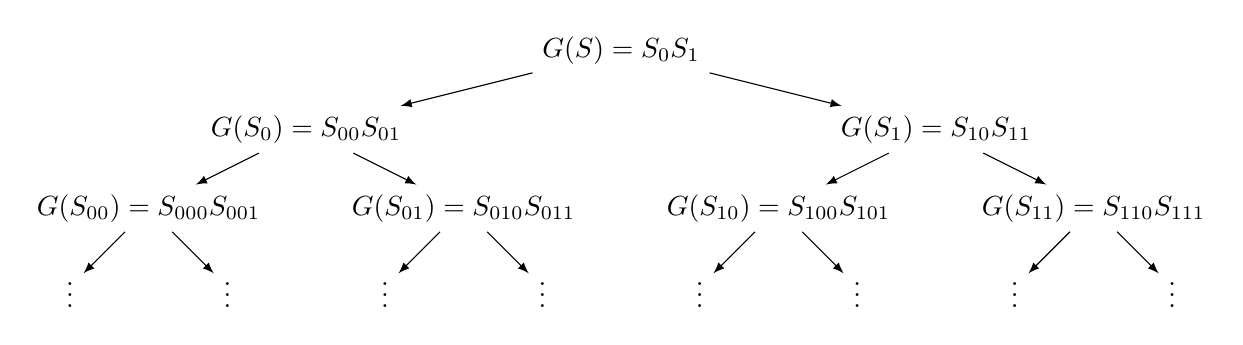
\begin{tikzpicture}[edge from parent/.style={draw,-latex}]
\node{\(G(S) = S_0S_1\)} [level distance=10mm,sibling distance=80mm]
child { node{\(G(S_0)=S_{00}S_{01}\)} [level distance=10mm ,sibling distance=40mm]
  child {node {\(G(S_{00})=S_{000}S_{001}\)}[level distance=10mm ,sibling distance=20mm]
    child {node {\(\vdots\)}}
    child {node {\(\vdots\)}}
  }
  child {node {\(G(S_{01})=S_{010}S_{011}\)}[level distance=10mm ,sibling distance=20mm]
    child {node {\(\vdots\)}}
    child {node {\(\vdots\)}}}
}
child { node{\(G(S_1)=S_{10}S_{11}\)} [level distance=10mm ,sibling distance=40mm]
  child {node {\(G(S_{10})=S_{100}S_{101}\)} [level distance=10mm ,sibling distance=20mm]
    child {node {\(\vdots\)}}
    child {node {\(\vdots\)}}
  }
  child {node {\(G(S_{11})=S_{110}S_{111}\)}[level distance=10mm ,sibling distance=20mm]
    child {node {\(\vdots\)}}
    child {node {\(\vdots\)}}}
};
\end{tikzpicture}
\end{center}

We continue this to depth \(n\), where we will have \(2^n\) leaf nodes. This gives us an array of \(2^n\) outputs which we can access according to some input/index \(i=b_1\cdots b_n\in[0,2^n)\) by traversing the binary tree according to \(b_1,\ldots,b_n\).

\subsubsection{Proof (skeleton) of Security}
We may prove that this PRF is secure in the sense outlined above by using a hybrid argument. Consider a tree similar to the one above, where every node contains a truly random \(2n\)-bit string. Then, consider each of the hybrid trees \(\mcH_k\) for \(k\in[0,n]\), where levels \(0,\ldots,k\) are truly random, and then the PRG \(G\) is applied to generate all of the levels after that.\medskip

Then, as usual, we assume that there is some distinguisher \(D\in\PPT\) which is able to tell apart the truly random tree \(\mcH_n\) and the PRF tree \(\mcH_0\) with non-negligible probability. It then follows by the triangle inequality that it should be able to tell apart at least two neighboring hybrids with non-negligible probability. \medskip

So, we create a new distinguisher \(D'\) using \(D\). \(D'\) receives, as input, some unknown distribution \(Z\). Then, \(D'\) guesses a \(k\in[1,n]\) and fills that level in the tree with samples from \(Z\). Everything above is filled with truly random strings, and everything below is generated from level \(k\) using \(G\). \smallskip

Then, suppose \(Z\) is the distribution generated by \(G\). Since the strings above it are completely random, it is easy to see that the resulting tree would correspond to \(\mcH_{k-1}\). And if \(Z\) is truly random, (i.e. \(\mcU_{2n}\)), then the resulting tree would correspond to \(\mcH_{k}\).\smallskip

So, when we feed this tree to \(D\), we have at least a \(\frac{1}{n}\) probability that we end up with a \(k\) which \(D\) can distinguish, and a non-negligible probability that \(D\) can properly distinguish at that \(k\). And, when \(D\) does distinguish properly, this means that \(D'\) was able to tell the difference between \(G\) and \(\mcU_{2n}\). So, we have used our PRF distinguisher to create a \(\PPT\) PRG distinguisher. So any adversary that breaks our PRF would also be able to break our PRG, meaning that this PRF is secure up to all the assumptions we have made up to this point.

\end{document}